% !TEX root = ../../buch.tex
% loesung.tex -- Beispiel-File für die Beschreibung der Loesung
%
% (c) 2020 Prof Dr Andreas Müller, Hochschule Rapperswil
%
\section{Lösung
\label{burgers:section:loesung}}
\rhead{Lösung}

Das Kaptiel \ref{chapter:pde}, beschreibt den theoretischen Aspekt der Numerik in Kombination mit partiellen Differentialgleichungen.
In diesem Abschnitt wird auf die numerischen Lösungsmethoden der Gleichung von Burgers eingegangen.


\subsection{Explizit}

Bei der Lösung der Gleichung mit dem expliziten Ansatz werden für die Berechnung des gewünschten Punktes $u_i^n$ auf Stellen eine  Zeitschritt in der Vergangenheit $u^{n-1}$ zurückgegriffen.
Folgend werden zwei Grundlegende Varianten mit jeweils einer kleinen Variation aufgezeigt.
 
\subsubsection{Lineare Methode 1}
	
	Diese Methode hat wohl den simpelsten Aufbau.
	Die Ableitung in der Zeit wird mit der Differenz der beiden Punkte $u_{i}^{n}-u_{i}^{n-1}$ realisiert.
	Wobei die Ableitung im Raum mit der Differenz $u_{i}^{n-1}-u_{i-1}^{n-1}$ abstrahiert wird.
	Sie wird grafisch in \ref{burgers:fig:Linear1} dargestellt.

	
	     \begin{figure}[!ht]
		\centering
		\includegraphics[height=.4\textwidth]{papers/burgers/BurgersEquation/tikz/Linear1/Linear1.pdf}
		\caption{Methode Explizit Linear1}
		\label{burgers:fig:Linear1}
		\end{figure}
	
	Die Grundlegende Gleichung \ref{burgers:eq_invisid_burgers} kann mit der gewählten Methode
	\begin{equation}
	  	\frac {\partial u}{\partial t}+u{\frac {\partial u}{\partial x}} = \frac{u_{i}^{n}-u_{i}^{n-1}}{\Delta t}+ u_{i}^{n}\, \frac{u_{i}^{n-1}-u_{i-1}^{n-1}}{\Delta x}=0
	  	  \label{burgers:eq_ex_lin1}
	  	\end{equation}
	  	
	  	umgeschrieben werden.
	  	Für den explizite Lösung muss \ref{burgers:eq_ex_lin} nach $ u_{i}^{n}$ aufgelöst werden.
	  	
	  	\begin{equation}
	  u_{i}^{n} = \frac{\Delta{x}\, u^{n-1}_{i}\,}{- \Delta{t}\, u^{n-1}_{i-1}\, + \Delta{t}\, u^{n-1}_{i}\, + \Delta{x}\,}
		  \label{burgers:eq_ex_sol_lin1}
	\end{equation}

	
	
\subsubsection{Lineare Methode 2}
	
	
	Für die Multiplikation des zweiten Bruches muss nicht unbedingt der gesuchte Punkt $u_{i}^{n}$ verwendet werden.
	Es kann auch der Punkt auf gleicher Stelle im Raum aber einen Zeitschritt in der Vergangenheit verwendet werden.
	
	
     \begin{figure}[!ht]
	\centering
	\includegraphics[height=.4\textwidth]{papers/burgers/BurgersEquation/tikz/Linear2/Linear2.pdf}
	\caption{Methode Explizit Linear2}
	\label{burgers:fig:Linear2}
	\end{figure}

	Wobei sich die Gleichung,
	\begin{equation}
			\frac {\partial u}{\partial t}+u{\frac {\partial u}{\partial x}} = \frac{u_{i}^{n}-u_{i}^{n-1}}{\Delta t}+ u_{i}^{n-1}\, \frac{u_{i}^{n-1}-u_{i-1}^{n-1}}{\Delta x}=0
		\label{burgers:eq_ex_lin2}
	\end{equation}
	 nur minimal ändert.
	 Auch kann wieder eine Lösung für den gesuchten Punkt gefunden werden.
	
	\begin{equation}
		u_{i}^{n} = \frac{u^{n-1}_{i}\, \left(\Delta{t}\, u^{n-1}_{i-1}\, - \Delta{t}\, u^{n-1}_{i}\, + \Delta{x}\,\right)}{\Delta{x}\,}
    	\label{burgers:eq_ex_sol_lin2}
	\end{equation}
	
\subsubsection{Stabilit\"atskriterium Lineare Methoden}
	Die Stabilit\"at kann f\"ur diese L\"osungsmethode nicht garantiert werden.
	Sie folgt dem Courant-Friedrichs-Lewy Kriterium
	
	
\subsubsection{Leap-Frog Methode 1}
	
	Bei genauer Betrachtungen von den Ableitungen in \ref{burgers:fig:Linear1} und \ref{burgers:fig:Linear2} erkennt man, dass sich die berechnete Ableitung eigentlich zwischen den beiden Punkten befindet.
	Theoretisch sollte man für ein optimales Resultat die Ableitung genau am Punkt $u_{i}^{n}$ erhalten.
	
	\medskip
	Die Leap-Frog Diskretisierung umgeht diese Problematik indem sie f\"ur die Ableitung einen Punkt \"uberspringt.
	Die daraus folgende L\"osung für die Ableitung befindet sich auf der gleichen Ebene im Raum wie der Punkt $u_{i}^{n}$, allerdings noch einen Zeitschritt zurück.
	In \ref{burgers:eq_ex_lf1} ist die Leap-Frog Methode grafisch dargestellt.
	
	
	\begin{figure}[!ht]
	\centering
	\includegraphics[height=.4\textwidth]{papers/burgers/BurgersEquation/tikz/Linear3/Linear3.pdf}
	\caption{Methode Explizit Leap-Frog 1}
	\label{burgers:fig:Linear3}
	\end{figure}
	
	Wiederum kann die Gleichung diskretisiert werden und nach dem gesuchten Punkt $u_{i}^{n}$ aufgel\"ost werden.
	
	\begin{equation}
		\frac {\partial u}{\partial t}+u{\frac {\partial u}{\partial x}} = \frac{u_{i}^{n}-u_{i}^{n-1}}{\Delta t}+ u_{i}^{n-1}\, \frac{u_{i+1}^{n-1}-u_{i-1}^{n-1}}{2\,\Delta x}=0
		\label{burgers:eq_ex_lf1}
	\end{equation}

	\begin{equation}
	 u_{i}^{n} = \frac{u^{n-1}_{i}\, \left(- \Delta{t}\, u^{n-1}_{i+1}\, + \Delta{t}\, u^{n-1}_{i-1}\, + 2 \Delta{x}\,\right)}{2 \Delta{x}\,}
		\label{burgers:eq_ex_sol_lf1}
	\end{equation}

\subsubsection{Leap-Frog Methode 2}
     \begin{figure}[!ht]
	\centering
	\includegraphics[height=.4\textwidth]{papers/burgers/BurgersEquation/tikz/Linear4/Linear4.pdf}
	\caption{Methode Explizit  Leap-Frog 2}
	\label{burgers:fig:Linear4}
	\end{figure}

	Wie schon in den bis Anhien gezeigten Varianten kann f\"ur die Multiplikation der Punkt $u_{i}^{n-1}$ verwendet werden.

	\begin{equation}
	\frac {\partial u}{\partial t}+u{\frac {\partial u}{\partial x}} = \frac{u_{i}^{n}-u_{i}^{n-1}}{\Delta t}+ u_{i}^{n}\, \frac{u_{i+1}^{n-1}-u_{i-1}^{n-1}}{2\,\Delta x}=0
	\end{equation}
	
	\begin{equation}
	u_{i}^{n} = \frac{2 \Delta{x}\, u^{n-1}_{i}\,}{\Delta{t}\, u^{n-1}_{i+1}\, - \Delta{t}\, u^{n-1}_{i-1}\, + 2 \Delta{x}\,}
	\end{equation}

\subsection{Stabilit\"atskriterium Leap-Frog Verfahren}
	Mit der Einf\"uhrung des Leap-Frog Verfahrens 









\subsection{Implizit}
\subsubsection{Leap-Frog Verfahren}

     \begin{figure}[!ht]
	\centering
	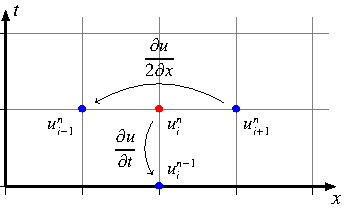
\includegraphics[height=.4\textwidth]{papers/burgers/BurgersEquation/tikz/implicit/implicit.pdf}
	\caption{Methode Implicit}
	\label{burgers:fig:Implicit}
\end{figure}

\begin{equation}
\frac {\partial u}{\partial t}+u{\frac {\partial u}{\partial x}} = \frac{u_{i}^{n}-u_{i}^{n-1}}{\Delta t}+ u_{i}^{n-1}\, \frac{u_{i+1}^{n}-u_{i-1}^{n}}{2\,\Delta x}=0
\end{equation}


\begin{equation}
    \frac{u_{i}^{n+1}-u_{i}^{n}}{dt} + u_{i}^{n} \, \frac{u_{i+1}^{n+1} - u_{i-1}^{n+1}}{2 \, dx} = 0
\end{equation}
\begin{equation}
  \frac{u_{i}^{n+1}-u_{i}^{n}}{dt} = -u_{i}^{n} \, \frac{u_{i+1}^{n+1} - u_{i-1}^{n+1}}{2 \, dx}
\end{equation}
\begin{equation}
  u_{i}^{n+1}-u_{i}^{n} = -u_{i}^{n} \, dt \, \frac{u_{i+1}^{n+1} - u_{i-1}^{n+1}}{2 \, dx}
\end{equation}
\begin{equation}
  u_{i}^{n+1} = -u_{i}^{n} \, dt \, \frac{u_{i+1}^{n+1} - u_{i-1}^{n+1}}{2 \, dx} + u_{i}^{n}
\end{equation}
\begin{equation}
2 \, dx \,  u_{i}^{n+1} = -u_{i}^{n} \, dt \, \left(u_{i+1}^{n+1} - u_{i-1}^{n+1} \right) + 2 \, dx \, u_{i}^{n}
\end{equation}
\begin{equation}
  2 \, dx \,  u_{i}^{n+1} + u_{i}^{n} \, dt \, u_{i+1}^{n+1} -u_{i}^{n} \, dt \, u_{i-1}^{n+1} =  2 \, dx \, u_{i}^{n}
\end{equation}


\begin{equation}
 -u_{i}^{n} \, dt \, u_{i-1}^{n+1} +  2 \, dx \,  u_{i}^{n+1} + u_{i}^{n} \, dt \, u_{i+1}^{n+1}=  2 \, dx \, u_{i}^{n}
\end{equation}



\begin{equation}
\left[{\begin{matrix}
{dx- u_{1}^{n}\, dt}&{ u_{1}^{n} \, dt}&{0}&{}&{0}\\[5pt]
{-u_{2}^{n} \, dt}&{ 2 \, dx}&{ u_{2}^{n} \, dt}&{}&{0}\\[5pt]
{0}&{-u_{3}^{n} \, dt}&{ 2 \, dx}&\ddots &{0}\\[5pt]
{0}&{0}&\ddots &\ddots &{ u_{M-1}^{n} \, dt}\\[5pt]
{0}&{0}&{}&{-u_{M}^{n} \, dt}&{dx + u_{1}^{M}\, dt}
\end{matrix}}
\right]\left[{\begin{matrix}
{ u_{1}^{n+1}}\\[5pt]
{ u_{2}^{n+1}}\\[5pt]
{ u_{3}^{n+1}}\\[5pt]
\vdots \\[5pt]
{ u_{M}^{n+1}}
\end{matrix}}\right]
=\left[{\begin{matrix}
{dx \, u_{1}^{n}}\\[5pt]
{ 2 \, dx \, u_{2}^{n}}\\[5pt]
{ 2 \, dx \, u_{3}^{n}}\\[5pt]
\vdots \\[5pt]
{dx \, u_{M}^{n}}
\end{matrix}}\right]
  \end{equation}

  \begin{equation}
    a_{i}x_{{i-1}}+b_{i}x_{i}+c_{i}x_{{i+1}}=d_{i}
  \end{equation}


  \begin{equation}
    \begin{bmatrix}{b_{1}}&{c_{1}}&{}&{}&{0}\\
      {a_{2}}&{b_{2}}&{c_{2}}&{}&{}\\
      {}&{a_{3}}&{b_{3}}&\ddots &{}\\
      {}&{}&\ddots &\ddots &{c_{n-1}}\\
      {0}&{}&{}&{a_{n}}&{b_{n}}\\
      \end{bmatrix}
      \begin{bmatrix}{x_{1}}\\
      {x_{2}}\\{x_{3}}\\\vdots \\
      {x_{n}}\\
      \end{bmatrix}
      =
      \begin{bmatrix}{d_{1}}\\
      {d_{2}}\\{d_{3}}\\
      \vdots \\{d_{n}}\\
    \end{bmatrix}
  \end{equation}

\begin{algorithm}\caption{Tridiagonal matrix algorithm (Thomas algorithm)}\label{TDMA}
  \setlength{\lineskip}{7pt}
  \begin{algorithmic}[1]
    \Function{Thomas}{$\textbf{a}, \textbf{b}, \textbf{c}, \textbf{d}$}
      \Comment{Vectors}
      \State $\hat c_1 \gets$ $ \dfrac{c_1}{b_1}$
      \State $\hat d_1 \gets \dfrac{d_1}{b_1}$
      \For{$i = 2,3,\dots,n-1$}
      \Comment{Forward sweep}
        \State $\hat c_i \gets \dfrac{c_i}{b_i-a_i \, \hat c_{i-1}}$
        \State $\hat d_i \gets \dfrac{d_i - a_i \, \hat d_{i-1}}{b_i-a_i \, \hat c_{i-1}}$
      \EndFor
      \State $x_n \gets \hat d_n$
      \For{$i = n-1,n-2,\dots,1$}
      \Comment{Backwards substitution}
        \State $x_i \gets \hat d_i - \hat c_i \, x_{i+1}$
      \EndFor
      \State \textbf{return} $\textbf{x}$
    \EndFunction
  \end{algorithmic}
\end{algorithm}


\subsubsection{Quadratisch}
     \begin{figure}[!ht]
	\centering
	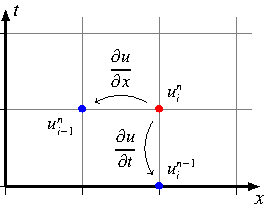
\includegraphics[height=.4\textwidth]{papers/burgers/BurgersEquation/tikz/quadratic/quadratic.pdf}
	\caption{Methode quadratic}
	\label{burgers:fig:quadratic}
\end{figure}

\begin{equation}
\frac {\partial u}{\partial t}+u{\frac {\partial u}{\partial x}} = \frac{u_{i}^{n}-u_{i}^{n-1}}{\Delta t}+ u_{i}^{n}\, \frac{u_{i}^{n}-u_{i-1}^{n}}{\Delta x}=0
\end{equation}

\begin{equation}
  u_{i}^{n} = \begin{bmatrix}
     \dfrac{\Delta{t}\, u^{n}_{i-1}\, - \Delta{x}\, - \sqrt{\Delta{t}\,^{2} \left(u^{n}_{i-1}\,\right)^{2} + 4 \Delta{t}\, \Delta{x}\, u^{n-1}_{i}\, - 2 \Delta{t}\, \Delta{x}\, u^{n}_{i-1}\, + \Delta{x}\,^{2}}}{2 \Delta{t}\,} \\[15pt]
     \dfrac{\Delta{t}\, u^{n}_{i-1}\, - \Delta{x}\, + \sqrt{\Delta{t}\,^{2} \left(u^{n}_{i-1}\,\right)^{2} + 4 \Delta{t}\, \Delta{x}\, u^{n-1}_{i}\, - 2 \Delta{t}\, \Delta{x}\, u^{n}_{i-1}\, + \Delta{x}\,^{2}}}{2 \Delta{t}\,}
  \end{bmatrix}
\end{equation}

\subsubsection{Linear}
     \begin{figure}[!ht]
	\centering
	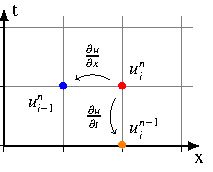
\includegraphics[height=.4\textwidth]{papers/burgers/BurgersEquation/tikz/linear5/linear5.pdf}
	\caption{Methode Implizit Linear}
	\label{burgers:fig:linear5}
	\end{figure}
	
	\begin{equation}
	\frac {\partial u}{\partial t}+u{\frac {\partial u}{\partial x}} = \frac{u_{i}^{n}-u_{i}^{n-1}}{\Delta t}+ u_{i}^{n-1}\, \frac{u_{i}^{n}-u_{i-1}^{n}}{\Delta x}=0
	\end{equation}
	
	\begin{equation}
	 u_{i}^{n} = \frac{u^{n-1}_{i}\, \left(\Delta{t}\, u^{n}_{i-1}\, + \Delta{x}\,\right)}{\Delta{t}\, u^{n-1}_{i}\, + \Delta{x}\,}
	\end{equation}